%%%%%%%%%%%%%%%%%%%%%%%%%%%%%%%%%%%%%%%%%%%%%%%%%%%%%%%%%%%%%%%%%%%%%%%%%%%%%%%
\documentclass[letterpaper, 10 pt, conference]{ieeeconf}  % Comment this line out
                                                          % if you need a4paper
%\documentclass[a4paper, 10pt, conference]{ieeeconf}      % Use this line for a4
                                                          % paper
\usepackage[utf8]{inputenc}  % Ng Edit for accents in spanish
\usepackage[spanish]{babel}  % Ng Edit for accents in spanish
\usepackage{hyperref}        % Ng Edit for adding urls
\usepackage{graphicx}        % Ng Edit for adding graphics
\usepackage{svg}
\IEEEoverridecommandlockouts                              % This command is only
                                                          % needed if you want to
                                                          % use the \thanks command
\overrideIEEEmargins
% See the \addtolength command later in the file to balance the column lengths
% on the last page of the document

\def\equationautorefname~#1\null{(#1)\null}%to use parenthesis in eqs.


% The following packages can be found on http:\\www.ctan.org
%\usepackage{graphics} % for pdf, bitmapped graphics files
%\usepackage{epsfig} % for postscript graphics files
%\usepackage{mathptmx} % assumes new font selection scheme installed
%\usepackage{times} % assumes new font selection scheme installed
%\usepackage{amsmath} % assumes amsmath package installed
%\usepackage{amssymb}  % assumes amsmath package installed

\title{\LARGE \bf
    Utilización de Múltiples Modelos de Redes Neuronales Convolucionales
    para la Detección de Rostros
}
\author{Pedro Luis González Roa, Pedro Oscar Pérez Murueta, Benjamín Valdés Aguirre,
José Antonio Cantoral Ceballos}

\begin{document}
    \maketitle
    \thispagestyle{empty}
    \pagestyle{empty}

    \begin{abstract}
        En los últimos años se ha demostrado la complejidad en la realización de
        algoritmos de detección y reconocimiento de rostros, ya que estos requieren de un alto
        nivel de abstracción porque existe un alto grado de similitud estructural entre los
        diferentes rostros. De esta manera, se requiere de la utilización de técnicas de
        \textit{deep learning}, cómo las \textit{redes neuronales convolucionales} (\textit{CNN}
        por sus siglas en inglés) para la extracción de características o \textit{features} que 
        proporciona una imagen.  Estas técnicas requieren de un modelo sumamente complejo y una
        base de datos de gran tamaño para un entrenamiento exitoso que desempeñe correctamente en
        diferentes situación de iluminación, calidad de la imagen, perfil de la cara, entre otros.
        Cumplir con las características previamente mencionadas significa una gran inversión de
        recursos, la cual sólo empresas de tamaños inmensos son capaces de invertir.
        Por lo que se propone utilizar una combinación de diferentes \textit{CNN}'s previamente
        entrenadas con diferentes arquitecturas y bases de datos.
        Se espera que las diferentes perspectivas o características extraidas por cada modelo
        sean capaces de complementarse entre sí para tener una representación más completa (aunque
        más compleja) del rostro a analizar sin la necesidad de entrenar un modelo de complejidad
        tan grande como la previamente mencionada. Finalmente se utilizará esta representación
        más compleja para determinar los grupos de imágenes de acuerdo a las diferentes personas
        en la base de datos.
    \end{abstract}

    \section{Antecedentes}

    \subsection{Extracción de Características en Imágenes}
    % Image Clustering
    El reconocimiento facial se encuentra directamente relacionado con uno de los
    problemas que ha recibido mucha atención en las últimas tres décadas. El problema
    de agrupamiento de imágenes, también conocido como \textit{Image Clustering (IC)}
    por sus siglas en inglés, se centra en obtener una representación numérica sobre
    una imagen y agruparla con imágenes que tienen representaciones similares.
    \cite{CombiningCNN}

    % CNN
    Métodos de \textit{deep learning}, cómo las \textit{redes neuronales convolucionales},
    utilizan una cascada de múltiples capas de unidades de procesamiento para extraer
    características específicas de las imágenes. Estas aprenden diferentes niveles de
    representación con cada capa de convolución que corresponden a los diferentes niveles
    de abstracción. Donde las primeras capas son capaces de reconocer y de detectar
    atributos de bajo nivel, similares a los modelos Gabor y SIFT (diseñados hace décadas);
    mientras que las capas más externas aprenden un nivel de abstracción más alto.
    Gracias a la variedad de niveles y filtros utilizados, los modelos de
    esta índole son capaces de tolerar a cierto nivel variaciones de ángulos,
    iluminación y calidad de la toma. \cite{Wang2021}

    \subsection{Reconocimiento de Rostros en la Actualidad}
    La detección de rostros consiste en tres fases principales:
    \begin{itemize}
        \item \textbf{Detección de rostro}: Aún cuando la detección de un rostro es trivial
            para los humanos, en términos de visión artificial no es una tarea sencilla. Esta
            tarea consiste en dado un vídeo o imágen, detectar y localizar un número
            desconocido de rostros (incluso si no hay alguno). Esta solución consiste en la
            segmentación, extracción y verificación de las posibles caras en un ambiente
            no controlado. \cite{FaceDetection2001}

        \item \textbf{Alineación del rostro}: Como segundo paso en este proceso, se alinea
            el rostro de acuerdo a coordenadas canónicas.\cite{Wang2021} Se han presentado
            varias propuestas que han sido evaluadas en previas investigaciones
            \cite{Zafeiriou2015}, de las cuales las \textit{CNN} han obtenido buenos resultados.
            Para el propósito de este proyecto, se utilizará la propuesta de Zhang \cite{MTCNN}.
            La cual utiliza una \textit{CNN} para la detección y la alineación de los rostros
            en la misma secuencia.

        \item \textbf{Reconocimiento}: Este último paso consiste en procesar el rostro obtenido
            en los pasos anteriores. Primero se procesa el rostro con algoritmos para validar
            si consiste de un rostro verdadero y no modificado. Esta parte del proceso se conoce
            como \textit{anti-spoofing}. Después se utiliza técnicas de \textit{deep learning} cómo
            \textit{CNNs} para extraer las características que distinguen un individuo de otro.
            Finalmente se compara con cada uno de los registros de la base de datos de las
            personas identificadas para buscar un emparejamiento.
            Este proceso puede ser descrito de la siguiente manera: \cite{Wang2021}
                \[ M(F(P(I_1)), F(P(I_2))) \]
            En donde \textit{$I_1$} e \textit{$I_2$} son las imágenes por procesar, \textit{$P$}
            es la función de preprocesamiento, \textit{$F$} es la función para obtener las
            características del rostro, y \textit{$M$} es el cálculo de la distancia entre
            ambas representaciones y consecuentemente la confirmación si es un emparejamiento.
    \end{itemize}
    La extracción de estas representaciones no es un procedimiento trivial. Incluso utilizando
    las técnicas más avanzadas de \textit{deep learning}, es muy probable que el modelo se vea
    afectado por cambios en el contexto de la imagen. Estos cambios pueden ser la utilización
    de artefactos como lentes o cubrebocas; diferentes perfiles de la cara en donde se aprecia
    porciones importantes del rostro; ó incluso diferentes niveles de iluminación y calidad de la
    imágen. \cite{Bodini2019}

    \section{Trabajos Relacionados}

    \subsection{Combinación de Redes Neuronales Convolucionales Previamente Entrenadas}
    Para obtener resultados exitosos en la agrupación de imágenes de mayor complejidad
    (cómo imágenes de objetos con estructuras complejas) es necesario la utilización
    de \textit{CNN}s previamente entrenadas para la extracción de características muy específicas,
    junto con algoritmos de \textit{deep clustering}. \cite{DCCS}\cite{JULE}\cite{Agarap2020}
    
    Existen una variedad de estos modelos \textit{CNN}, los cuales tienen un mismo objetivo pero
    aportan una perspectiva diferente gracias a variaciones dentro de las arquitecturas, funciones
    de activación y/ó base de datos utilizada para el entrenamiento. Para casos específicos un
    modelo puede tener mejor desempeño que otro en la obtención de características definitivas,
    pero en otro contexto puede tener un desempeño inferior. Guérin y coautores en la investigación
    \textit{'Combining pretrained CNN feature extractors to enhance clustering of complex natural images'}
    utilizan diferentes modelos \textit{CNN} para obtener resultados más constantes en la tarea de
    agrupación de imágenes complejas. Esto es gracias a que no se puede saber el modelo óptimo para
    cualquier situación (al menos de que se prueben todos), y al combinar diferentes modelos se
    obtiene una representación más completa y compleja. Esto es sacrificando una rápida respuesta
    a cambio de un resultado más fiable.\cite{CombiningCNN}


    \subsection{Modelo IE-CNN}
    An-Pint Song comprobó en su investigación \textit{'Similar Face Recognition Using the IE-CNN
    Model'} la importancia de tomar múltiples perspectivas sobre una misma imágen al realizar el
    reconocimiento de rostros.\cite{IECNN} Este artículo menciona un fenómeno dentro de la
    investigación para el desarrollo de modelos de reconocimiento: siempre se utiliza la parte
    interna del rostro para el entrenamiento de los modelos. Lo cual no se apega completamente
    a cómo los humanos procesamos un nuevo rostro. Cuando es difícil determinar la comparación
    entre individuos, incrementamos nuestro enfoque en características específicas de la cara
    para discernir entre los dos rostros diferentes.\cite{Young1987}\cite{Andrews2010}
    Por lo que Song propone un modelo de \textit{CNN} que utiliza diferentes perspectivas
    enfocadas en partes estratégicas del rostro para obtener una representación mejorada.
    La cual obtuvo una mejora en los resultados de alrededor del 5\%.\cite{IECNN}

    \section{Planteamiento del Problema}
    % Diferentes situaciones afectan la fiabilidad de los modelos cnn
    Reiterando la problemática previamente mencionada sobre la utilización de \textit{CNN},
    la extracción de las características únicas de una cara para el reconocimiento facial
    es un reto no trivial por múltiples factores. Uno de estos es la posición del rostro,
    ya que es posible ocultar atributos clave que conllevan a una recolección incompleta
    de la información necesaria. Así mismo, el uso de artefactos como lentes o cubrebocas
    llevan a obstrucciones en dicha recolección. Por otro lado, las expresiones faciales
    pueden alterar la representación numérica, incluso cuando es el rostro del mismo individuo.
    Finalmente, los últimos factores que afectan son relacionados al ambiente, cómo la iluminación
    y la calidad de la cámara. \cite{Bodini2019}

    El diseño y entrenamiento de modelos lo suficientemente complejos que puedan desempeñarse
    correctamente en cualquier tipo de contexto requieren de una gran cantidad de recursos de
    \textit{hardware} y de una base de datos que incluya varias representaciones por cada uno
    de estos contextos. Incluso corporaciones gigantes han tenido problemas para resolver esta
    problemática en todos los casos posibles. Podemos tomar como ejemplo la situación en la que
    se encontró Apple, cuando su reconocimiento facial en sus dispositivos \textit{iphone} no
    era capaz de discernir correctamente entre individuos del país chino. \cite{Birchall2017}


    \section{Propuesta}
    % Modelo con mayor fiabilidad a coste de tiempo o utilización de hardware

    \subsection{Descripción de la propuesta}
    En esta investigación se propone utilizar múltiples modelos de redes neuronales convolucionales
    (\textit{CNN}) en combinación para obtener una representación de mayor complejidad pero de
    mayor precisión. Al igual que el modelo de Guérin \cite{CombiningCNN} se espera un aumento 
    en el tiempo de ejecución del programa, pero se busca resultados constantes durante contextos
    diferentes provenientes de bases de datos públicas.

    Considerando que para determinar si un rostro pertenece a la misma persona, es decir se
    calcula la distancia entre las representaciones numéricas y se compara en contra de un
    threshold previamente determinado, se propone utilizar algoritmos de agrupamiento
    (\textit{clustering}) para realizar un mapa de las diferentes representaciones para cada
    rostro. De esta manera no es necesario comparar el rostro desconocido con cada una de las
    imágenes identificadas; sólo se predicirá el \textit{cluster} a cual pertenece y que se
    mantenga dentro de una distancia definida. En caso de que se encuentre fuera de la distancia
    definida se considera a la imágen cómo un nuevo individuo a registrar.

    Para el desarrollo de esta investigación, se utilizó la librería de Python
    \textit{Keras-VGGFace}, la cual contiene modelos previamente entrenados con las arquitecturas
    \textit{VGG16}, \textit{RESNET50}, \textit{SENET50}. Aunque hay más modelos públicos
    \cite{Inceptionv3}\cite{Facenet}, se decidió realizar las pruebas con estos tres modelos.

    \subsection{Concatenación de Diferentes Representaciones (CC)}
    El acercamiento de concatenación consiste en, cómo su nombre lo dice, concatenar las
    diferentes representaciones obtenidas de cada modelo. En otras palabras, se agregan dimensiones
    por cada modelo que proporciona una perspectiva.
    
    Ya que se espera que entre más modelos utilizados la complejidad de tiempo crezca
    exponencialmente, se evaluará el desempeño del algoritmo de reducción de dimensiones
    \textit{Principal Component Analysis (PCA)} para reducir el tiempo de procesamiento sin
    que exista un impacto en la precisión del modelo.

    \begin{figure}[ht]
        \centering
        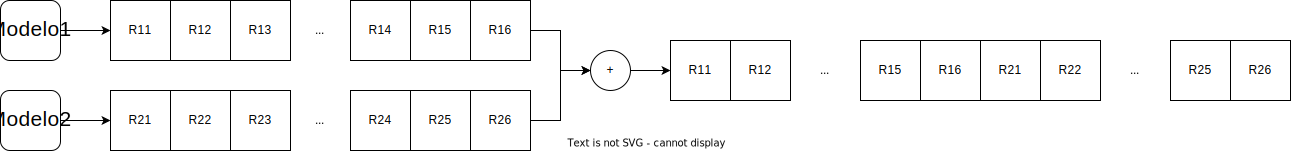
\includegraphics[width=8cm]{./figs/cc.png}
        \label{fig: Concatenación}
        \caption{Representación visual del acercamiento de concatenación.}
    \end{figure}

    % Por qué CC

    \subsection{Utilización de Métodos de Consenso de Agrupamiento (MVEC)}
    Existen diferentes algoritmos e implementaciones para el agrupamiento de información. Aunque
    haya una gran variedad de estos algoritmos, muchos de estos encuentran soluciones apropiadas
    pero no óptimas. Estos convergen a un óptimo local y no a un óptimo global, aunque existe
    la pequeña posibilidad de que algunos sí llegan a este último (cómo por ejemplo: el algoritmo
    de \textit{k-means}). Ya que llegar a una solución óptima global es un poco aleatoria por la
    dependencia de la inicialización y distribución de las diferentes entradas, escoger un
    algoritmo de agrupación apto para la información presentada puede ser una tarea difícil. Para
    solucionar este problema, diferentes investigadores introdujeron el concepto de métodos de
    conjuntos para agrupamientos (\textit{Cluster Ensembles - CE} por sus siglas en inglés),
    ó también conocidos como métodos de consenso de agrupamiento (\textit{Consensus Clustering}).
    Los algoritmos de \textit{CE} combinan los diferentes resultados de agrupamiento para generar
    un agrupamiento final, sin necesitar acceso a los algoritmos o registros de información.
    \cite{Golalipour2021}

    \begin{figure}[ht]
        \centering
        \includegraphics[width=8cm]{./figs/mvec.png}
        \label{fig: MVEC}
        \caption{Representación visual del acercamiento de consenso.}
    \end{figure}

    % Por qué MVEC

    Para el enfoque de este proyecto, utilizaremos la librería de Python proporcionada por Sano
    Takehiro \cite{Sano_ClusterEnsembles_2021}; con el algoritmo de \textit{Hybrid Bipartite Graph
    Formulation}. \cite{Fern2004}

    \subsection{Utilización de Agrupamiento de Múltiples Vistas (MVC)}
    En la era de \textit{Big Data}, se obtienen perspectivas diferentes de un mismo objeto desde
    una gran variedad de sensores. Estos sensores producen una salida de diferentes características
    entre sí, es decir son perspectivas que se complementan entre ellas para una representación
    más compleja del objeto observado. Por lo cual, ha surgido una tendencia a experimentar con
    algoritmos que puedan utilizar las diferentes dimensiones de cada vista para hacer predicciones
    más certeras.  Gracias a la necesidad de identificar diferentes objetos en una gran cantidad de
    información y vistas, ha incrementado en popularidad los Algoritmos de Agrupación de Vistas
    múltiples; \textit{Multi-View Clustering (MVC)} en inglés.

    Cómo se mencionó previamente, cada vista puede considerarse como un mundo diferente afectado
    por diferentes variables. Esta exhibición de propiedades heterogéneas contiene un potencial de
    contener posibles conecciones entre ellas, las cuales pueden ser explotadas para desenmascarar
    características únicas de cada objeto. La idea principal de utilizar \textit{MVC} es
    particionar objetos de acuerdo a diferente criteria relacionada con estas conecciones de sus
    diferentes vistas, ajustando algoritmos comunes y conocidos (cómo \textit{k-means}) para un
    enfoque de mayor complejidad. \cite{Yang2018}

    Las pruebas realizadas en esta investigación utilizarán la librería de Python \textit{MVLearn}.
    \cite{MVlearn} La cual contiene mayor variedad de algoritmos de múltiples vistas para utilizar.
    Cabe mencionar que por las restricciones de este proyecto, sólo se utilizó el algoritmo de
    \textit{Multi-view K-Means Clustering}.

    % Cómo se relaciona

    \subsection{Medición y Datasets}
    % NMI
%    Para evaluar el desempeño de este modelo de combinación se dividirá en dos etapas dicha
%    evaluación:
%    \begin{enumerate}
%        \item Se dará la tarea de agrupar las imágenes de un número conocido y variable de
%            personas. La composición de estos grupos será evaluada con la métrica
%            \textit{Normalized Mutual Info (NMI)} \cite{NMI}. Es importante esta puntuación porque
%            al evaluar la facilidad para el algoritmo de determinar los grupos de acuerdo a las
%            diferentes representaciones significa que estas se encuentran separadas de las
%            representaciones de rostros de otros individuos y también se encuentran cercanas a las
%            representaciones de un mismo individuo por lo que se cumple nuestra hipótesis de una
%            representación más completa de las características únicas del rostro.
%        \item De un mapeo previamente realizado de un número conocido de personas, se agregarán
%            más imágenes de personas incluidas en dicho agrupamiento y de otras no incluidas. Por
%            cada imágen se evaluará si predijo correctamente la persona a la que pertenece o si
%            es una persona nueva. Denotando el porcentaje de casos de falsos positivos,
%            ya que es una métrica importante en los sistemas de seguridad biométricos.
%        \item La diferencia de tiempo para realizar el agrupamiento entre cada uno de los
%            acercamientos.
%    \end{enumerate}
    Para evaluar el desempeño de este modelo de combinación, se dará la tarea de se dará la
    tarea de agrupar las imágenes de un número conocido y variable de personas. La composición
    de estos grupos será evaluada con la métrica \textit{Normalized Mutual Info (NMI)}
    \cite{NMI}. Es importante esta puntuación porque al evaluar la facilidad del algoritmo para
    determinar los grupos de acuerdo a las diferentes representaciones significa que estas se
    encuentran separadas de las representaciones de rostros de otros individuos y también se
    encuentran cercanas a las representaciones de un mismo individuo; por lo que se cumple
    nuestra hipótesis de una representación más completa de las características únicas del
    rostro.

    % Datasets
    Es importante que estas evaluaciones sean hechas con la mayor cantidad posible de imágenes que
    representen los diferentes contextos que afectan a este tipo de autenticación biométrica. Por
    lo que se decidió utilizar cuatro diferentes \textit{datasets} públicas:
    \begin{itemize}
        \item \textbf{Yale Face Dataset}: Esta base de datos pública es una de las más comunes y
            utilizadas para investigación, validación de modelos de detección y reconocimiento de
            rostros. Esta consiste de un total de 165 imágenes de 15 individuos con diferentes
            ángulos de iluminación, posición de rostro y utilización de lentes. Este dataset se
            utilizó para realizar pruebas sencillas durante el desarrollo del modelo propuesto.
%        \item \textbf{The Extended Yale Face Dataset B}\cite{YaleDataset}: Este \textit{dataset}
%            consiste en 16,128 imágenes en escala de gris de 28 individuos. Cada uno tiene 9
%            posiciones de rostro, y 64 situaciones diferentes de iluminación. Este dataset se
%            utilizará para experimentar los cambios de iluminación y posición de rostro.
        \item \textbf{CelebA Dataset}\cite{CELEBA}: Consiste en 10,177 individuos con un total de
            202,599 imágenes de rostros. Se recomienda este dataset porque tiene al menos dos o más
            imágenes por cada una de las personas; lo cual es excelente para probar que las
            representaciones de un mismo individuo no tengan mucha distancia entre ellas.
        \item \textbf{Labeled Faces in the Wild (LFW)}\cite{LFW}: Al igual que la base de datos de
            Yale, \textit{LFW} es muy utilizado en investigaciones. Este \textit{dataset} cuenta
            con 13,233 imágenes de 5,749 individuos. La desventaja de este dataset es que sólo
            1,680 individuos tienen dos o más imágenes.
        \item \textbf{Masked Labeled Faces in the Wild (MLFW)}\cite{MLFW}: Consiste en modificar el
            \textit{dataset LFW}, agregando una imagen de un cubrebocas para cada rostro. Por lo
            que se buscará aprovechar este dataset para probar la consistencia del modelo frente
            a situaciones inesperadas, cómo lo es una limitación visual para la parte inferior del
            rostro.
    \end{itemize}

    \section{Resultados}
    Al analizar los grandes tamaños de cada \textit{dataset}, se observó que no es viable realizar
    análisis sobre todas las imágenes de cada uno en un mismo análisis por limitaciones de memoria.
    En esta investigación buscamos comprobar nuestra hipótesis sobre la utilización de diferentes
    modelos \textit{CNN} es capaz de construir una representación más completa de un individuo.
    En otras palabras, buscamos que las representaciones de cada rostros sean sencillas de
    identificar y agrupar; no buscamos determinar si es posible agrupar una base de datos de
    imágenes tan extenso. Para solucionar este problema que ocasiona utilizar
    tanta memoria, optamos por realizar múltiples pruebas de al menos 50 individuos por
    \textit{dataset} (con la excepción del \textit{Yale dataset} porque cuenta con 15 individuos).

    Una vez específicado el tamaño de las pruebas, organizamos la experimentación de este proyecto
    en dos pasos, cada uno con un objetivo diferente:

    \subsection{Resultados entre los diferentes algoritmos de agrupación}
    Cómo primer paso en la implementación de esta investigación se buscó un algoritmo de agrupación
    que fuera capaz de obtener resultados constantes. Por lo que se realizaron 100 pruebas de
    alrededor de 50 personas por \textit{dataset} para evaluar tres tipos de algoritmos de
    agrupación.

    \begin{itemize}
        \item \textbf{\textit{k-means}}: Se escogió este algoritmo por la idea de que si se
            encuentra una representación general de un rostro (el \textit{centroide}) es más
            sencillo encontrar representaciones cercanas a esta representación general de un
            individuo.
        \item \textbf{\textit{agglomerative}}: Como segunda opción se experimentó con
            \textit{agglomerative clustering} por ser un algoritmo de agrupación jerárquica. Por lo
            que se tendrá un resultado determinístico.
        \item \textbf{\textit{multiview k-means}}: Este es el algoritmo elegido para evaluar el
            acercamiento de Agrupamiento de Múltiples Vistas.
    \end{itemize}

    Ya que se espera la necesidad de trabajar con una gran cantidad de información en muy poco
    tiempo, también se aprovecharon estas pruebas para determinar si al utilizar un reductor de
    dimensionalidad se ve afectado el puntaje de los grupos obtenidos.

    \begin{figure}[ht]
        \centering
        \includegraphics[width=8cm]{./figs/cluster_comparison.png}
        \label{fig: Results Cluster}
        \caption{Análisis de resultados por algoritmo de agrupamiento.}
    \end{figure}

    La figura 3 nos ayuda a visualizar la variación de los resultados preliminares que se
    obtuvieron para resolver el primer objetivo. Con esta información podemos hacer
    las siguientes reflexiones:

    \begin{enumerate}
        \item El acercamiento de Agrupamiento de Múltiples Vistas no es viable porque tiende a
            tener los mismos resultados a cuando se realiza agrupamientos de forma aleatoria.
            Al analizar los archivos de salida, se puede ver que por la complejidad del algoritmo
            en todos los casos converge a un mínimo local que no es óptimo porque sólo se logra
            encontrar una menor cantidad de grupos antes de converger.
        \item Existe poca diferencia entre los resultados de los algoritmos \textit{k-means} y
            \textit{agglomerative}. Por lo que se decidió optar por utilizar el algoritmo de
            \textit{k-means}, ya que este almacena los \textit{centroides} que se utilizarían
            en el modelo para determinar si una nueva imagen es parte del grupo de representaciones
            del mismo rostro.
        \item Finalmente utilizar un reductor de dimensionalidad, \textit{PCA}, no
            altera la precisión al agrupar las imágenes. Por lo tanto, se utilizará este reductor
            de dimensiones para las siguientes pruebas que contienen un número mucho mayor de
            imágenes.
    \end{enumerate}
    % Fracaso mvc (Comparación de modelos de agrupamiento)
    % Resultados y consistencia de CC

    \subsection{Resultados de desempeño en agrupación de acuerdo al dataset}
    Se determinó que nuestro siguiente objetivo era medir la puntuación \textit{NMI} para la
    agrupación de las imágenes en pruebas de más de 100 individuos. Haciendo énfasis en las
    diferentes características de cada dataset para realizar reflexiones de estas.

    \begin{figure}[ht]
        \centering
        \includegraphics[width=8cm]{./figs/singles.png}
        \label{fig: Results Single}
        \caption{Análisis de resultados de los modelos sin combinación.}
    \end{figure}

    \begin{figure}[ht]
        \centering
        \includegraphics[width=8cm]{./figs/dataset_comparison.png}
        \label{fig: Results Dataset}
        \caption{Análisis de resultados por \textit{dataset}.}
    \end{figure}

    Al reflexionar sobre los diferentes resultados de cada dataset de acuerdo a la
    figura 5, reflexionamos sobre los siguientes puntos:
    \begin{enumerate}
        \item \textbf{Dataset CelebA}: A primera vista los resultados que se obtuvieron en todos
            los tipos de acercamiento dejaron mucho que desear. Aunque en la
            figura 6, en la cual se hace una comparación de los resultados cuando se utiliza
            la arquitectura \textit{VGG16} en combinación con otras, podemos ver que se mantiene
            el nivel de precisión de este modelo. Al tener un puntaje promedio de 0.82 de forma
            individual, el modelo \textit{VGG16} proporciona las características más definitivas de
            los rostros en este dataset. En contraste, las otras dos arquitecturas -
            \textit{RESNET} y \textit{SENET} - no tienen una perspectiva lo suficientemente clara
            para determinar con precisión los grupos. Al utilizar el algoritmo de concatenación,
            las características de la mejor red neuronal son compartidas para que se obtenga un
            mejor resultado.
            \begin{figure}[ht]
                \centering
                \includegraphics[width=8cm]{./figs/celeba_vgg.png}
                \label{fig: Results Celeba with VGG}
                \caption{Análisis de resultados en \textit{celeba} cuando se utiliza VGG.}
            \end{figure}
        \item \textbf{Dataset MLFW}: Al analisar la figura 4, nos podemos percatar que es el único
            dataset en el que la arquitectura \textit{VGG16} no obtuvo los mayores resultados.
            Este dataset oculta la parte inferior del rostro, por lo que se puede suponer que en
            esta zona hay características de las que depende esta arquitectura para discernir entre
            rostros.  Aunque en la figura 5, podemos observar que se obtienen mejores resultados
            gracias a que las otras arquitecturas tienen una perspectiva que complementa a las
            predicciones de esta.
    \end{enumerate}

%    \subsection{Resultados de desempeño en falsos positivos}
%    \begin{figure}[ht]
%        \centering
%        \includegraphics[width=8cm]{./figs/dataset_comparison.png}
%        \label{fig: Results FP}
%        \caption{Análisis de resultados de acuerdo a los falsos positivos.}
%    \end{figure}

%    \subsection{Resultados en medición de tiempo}
% Faltó tiempo para una nueva foto individual
%    \begin{figure}[ht]
%        \centering
%        \includegraphics[width=8cm]{./figs/dataset_comparison.png}
%        \label{fig: Results Map Time}
%        \caption{Análisis de resultados de acuerdo al tiempo de agrupación.}
%    \end{figure}

    \section{Conclusiones}
    En el estado del arte de reconocimiento de rostros se ha popularizado la implementación de
    \textit{CNN} para la extracción de las características únicas que identifican a un individuo.
    Esta técnica de \textit{deep learning} se ve afectada directamente por las decisiones
    arbitrarias del programador al realizar el diseño de esta, por lo que hay una gran variación
    de resultados (incluso con las mismas arquitecturas) en diferentes casos de prueba. En este
    artículo se propone la idea de aprovechar las diferentes perspectivas que tienen cada uno de
    los modelos \textit{CNN} para tener una perspectiva más completa.

    Con los resultados y sus reflexiones previamente mencionadas, podemos concluir que en caso de
    necesitar un modelo que tenga la flexibilidad para la detección de rostros en una gran
    variedad de contextos es posible utilizar una combinación de redes neuronales previamente
    entrenadas. Aunque existe la posibilidad de que se seleccione una \textit{CNN} entrenada
    con un dataset parecido al contexto que se somete y que puede incluso tener el mejor resultado
    a comparación de otras redes, también existe la posibilidad de elegir una red neuronal que
    no es apta para la situación que se presenta. Por lo que al sacrificar tiempo para dedicarlo a
    la ejecución de los diferentes modelos, podemos combinar las diferentes perspectivas para
    obtener un resultado más constante.

    \section{Futuras Aportaciones}
    En este artículo se realizaron pequeños pero múltiples experimentos para demostrar que es
    posible combinar diferentes perspectivas en busca de una visión más amplia. Se obtuvieron
    resultados positivos, incluso cuando sólo se utilizaron tres arquitecturas - \textit{VGG16},
    \textit{RESNET50} y \textit{SENET50}. Existe la posibilidad de que se puedan utilizar
    otras arquitecturas diferentes y encontrar una mayor complementación entre ellas.

    Así mismo, cabe mencionar que se experimentó con una pequeña cantidad de algoritmos de
    agrupamiento; de los cuales existen una mayor variedad (incluso cuando se trata de
    agrupamiento de múltiples vistas). En un artículo relacionado, Guerín obtuvo resultados
    muy altos en \textit{datasets} selectos con el algoritmo de \textit{deep clustering} llamado
    \textit{Joint Unsupervised Learning of Deep Representations and Image Clusters} \cite{JULE};
    con el cual se puede expandir esta experimentación.

    Finalmente, se propone experimentar más sobre el comportamiento de estas combinaciones de
    modelos frente a imágenes nuevas después de haber realizado el agrupamiento inicial. Esto
    con el objetivo de evaluar a un nivel más profundo las capacidades de autenticación biométrica.
    % Utilizar más modelos como Inception
    % Deep Learning Clustering JULE
    % Entrenar modelos tapando partes estratégicas de la cara

    \bibliographystyle{ieeetr} % We choose the "plain" reference style
    \bibliography{refs} % Entries are in the refs.bib file
\end{document}
